\documentclass{Exams}
\usepackage{preamble}
\usepackage{fancyhdr}
\usepackage{mathrsfs}
\usepackage{upgreek}
\usepackage{graphicx}
\usepackage{wrapfig}
\usepackage{indentfirst}
\usepackage[strict]{changepage}
\pagestyle{fancy}

%   Используйте для теоремы окружение 
%   \begin{theorem}[name] \end{theorem}
%   Аналогично:
%   определение (definition)
%   лемма (lemma),
%   следствие (corollary)
%   пример (example)
%   замечание (remark)
%   док-во (Proof) (именно с большой буквы)

% \Nat - множество натуральных чисел
% \Real - множество вещественных чисе
% \Zint - множество целых чисел
% \Complex - множество комплексных чисел
% \eps - эпсилон  
\fancyhead[RO]{\slshape А. Орехова \rightmark}
\fancyfoot[C]{\thepage}

\author{}
\title{Билеты к экзамену}
\date{2023}
\begin{document}

\subject{Математическая логика}
\ExamMakeTitle
\tableofcontents

\section{Логические операции над высказываниями}
\subsection*{Логика высказываний}
\begin{definition}
    \textit{Высказыванием} называется повествовательное предложение, о котором можно
    судить, истинное оно или ложное.

    Обозначаются высказывания: A, B, C...
\end{definition}

\begin{definition}
    \textit{Истинностное значение} высказывания А обозначается символом $\lambda(A)$ и определяется по формуле:

    $\lambda(A) = 1$, если высказывание А истинно

    $\lambda(A) = 0$, если высказывание А ложно
\end{definition}

\subsection*{Алгебра высказываний}
Из высказываний путем соединения их с помощью связок <<не>>, <<и>>, <<или>>, <<следует>>, <<равносильно>> можно составлять новые, более сложные высказывания.

При этом главное внимание уделяется функциональным зависимостям истинностных значений высказываний, в которых истинность или ложность новых высказываний определяется истинностью или ложностью составляющих их высказываний.

\begin{definition}
    \textit{Отрицанием высказывания А} называется высказывание $\lnot A$ (читается <<не $А$>>), которое истинно в том и только том случае, если высказывание $A$ ложно.
\end{definition}
Таблица истинностных значений операции отрицания:

\begin{center}
    \begin{tabular}{|c|c|}
    \hline
    $A$ & $\lnot A$ \\ \hline
    1   & 0         \\ \hline
    0   & 1         \\ \hline
    \end{tabular}
\end{center}

\begin{definition}
    \textit{Конъюнкцией высказываний A, B} называется высказывание $A\land B$ (читается <<$A$ и $B$>>), которое истинно в том и только том случае, если оба высказывания $A$, $B$ истинны.
\end{definition}

\begin{definition}
    \textit{Дизъюнкцией высказываний A, B} называется высказывание $A\lor B$ (читается <<$A$ или $B$>>), которое ложно в том и только том случае, если оба высказывания A, B ложны.
\end{definition}

\begin{definition}
    \textit{Импликацией высказываний A, B} называется высказывание $A\Rightarrow B$ (читается <<$A$ влечет $B$>>), которое ложно в том и только том случае, если высказывание $A$ истинно, а высказывание $B$ ложно.
\end{definition}

\begin{definition}
    \textit{Эквивалентностью высказываний A, B} называется высказывание $A\Leftrightarrow B$ (читается <<$A$ равносильно $B$>>), которое истинно в том и только том случае, если высказывания $A$ и $B$ имеют одинаковое истинностное значение.
\end{definition}

Таблица истинностных значений логических операций:
\begin{center}
    \begin{tabular}{|c|c|c|c|c|c|}
        \hline
        $A$ & $B$ & $A\land B$ & $A\lor B$ & $A\Rightarrow B$ & $A\Leftrightarrow B$ \\ \hline
        0   & 0   & 0          & 0         & 1                & 1                    \\ \hline
        0   & 1   & 0          & 1         & 1                & 0                    \\ \hline
        1   & 0   & 0          & 1         & 0                & 0                    \\ \hline
        1   & 1   & 1          & 1         & 1                & 1                    \\ \hline
        \end{tabular}
\end{center}

\begin{definition}
    \textit{Алгеброй высказываний} называется множество всех высказываний $\mathscr{P}$ с логическими операциями $\lnot $, $\land $, $\lor $, $\Rightarrow $, $\Leftrightarrow $.
\end{definition}

\section{Формулы и истинностные значения формул}
\subsection*{Формулы алгебры высказываний}
\begin{definition}
    Свойства алгебры всказываний $\mathscr{P}$ описываются с помощью формул, которые строятся из переменных символов с помощью знаков логических операций. Такие формулы принято называть также \textit{пропозициональными формулами}.
\end{definition}

\begin{definition}
    Символы логических операций $\lnot$, $\land$, $\lor$, $\Rightarrow$, $\Leftrightarrow$, которые называются \textit{пропозициональными связками}.
\end{definition}

\begin{definition}
    Переменные символы $X, Y, Z,\dots$, которые используются для обозначения высказываний, называются \textit{пропозициональными переменными}.
\end{definition}

\begin{definition}
    \textit{Формулы} алгебры высказываний индуктивно определяются по правилам:

    \begin{enumerate}
        \item Каждая пропозициональная переменная является формулой
        \item Если $\Phi$, $\Uppsi$  формулы, то формулами являются также выражения
        ($\lnot\Phi$), ($\Phi\land\Uppsi$), ($\Phi\lor\Uppsi$), ($\Phi\Rightarrow\Uppsi$), ($\Phi\Leftrightarrow\Uppsi$)
    \end{enumerate}

Множество всех формул алгебры высказываний обозначим $\mathcal{F}_{AB}$
\end{definition}

Для упрощения записи формул скобки в них по возможности опускаются с учетом следующего \textbf{приоритета выполнения операций:} $\lnot, \land, \lor$ и остальные.

Так, формула $((((\lnot X)\land (\lnot Y))\lor(\lnot(\lnot Z)))\Rightarrow(X \lor (\lnot Y)))$
сокращенно записывается в виде $\lnot X \land Y \lor \lnot\lnot Z \Rightarrow X \lor \lnot Y$.

Если в формулу $\Phi$ входят переменные $X_1, \dots, X_n$, то записывают $\Phi = \Phi(X_1,\dots,X_n)$.

Из индуктивного опеределения формул следует, что если в формулу $\Phi$ вместо переменных $X_1,\dots,X_n$ подставить произвольные конкретные высказывания $A_1,\dots,A_n$, то получится некоторое сложное высказывание $\Phi(A_1,\dots,A_n)$.

Истинностное значение высказывания $\lambda(\Phi(A_1,\dots,A_n))$ определяется истинностными значениями исходных высказываний $\lambda(A_1),\dots,\lambda(A_n)$ согласно таблицам истинностных значений логических операций $\lnot $, $\land $, $\lor $, $\Rightarrow $, $\Leftrightarrow $.

Формула $\Phi$ определяет функцию $n$ переменных $F_\Phi$, которая каждому упорядоченному набору $(\lambda(X_1),\dots,\lambda(X_n))$ $n$ элементов множества {0,1} ставит в соответствие элемент $\lambda(\Phi(X_1,\dots,X_n))$ этого же множества.

\begin{definition}
    Функция $F_\Phi$ называется \textit{истинностной функцией формулы $\Phi$} и графически представляется \textit{истинностной таблицей}.

    Такая таблица содержит $2^n$ строк и имеет ожно из возможных $2^{2^n}$ возможных распределений 0 и 1 в последнем столбце.
\end{definition}

\begin{example}
    Составим таблицу истинности для формулы 
    
    $(P\Rightarrow Q) \Leftrightarrow (\lnot Q \Rightarrow \lnot P)$

    \begin{center}
        \begin{tabular}{|c|c|c|c|c|c|c|}
            \hline
            $P$ & $Q$ & $P \Rightarrow Q$ & $\lnot Q$ & $\lnot P$ & $\lnot Q \Rightarrow \lnot P$ & $(P\Rightarrow Q)\Leftrightarrow (\lnot Q \Rightarrow \lnot P$) \\ \hline
            0   & 0   & 1                 & 1         & 1         & 1                             & 1                                                              \\ \hline
            0   & 1   & 1                 & 0         & 1         & 1                             & 1                                                              \\ \hline
            1   & 0   & 0                 & 1         & 0         & 0                             & 1                                                              \\ \hline
            1   & 1   & 0                 & 0         & 0         & 1                             & 1                                                              \\ \hline
            \end{tabular}
    \end{center}

    Таблица показывает, что какого бы истинностного значения высказывания ни подставлялось в данную формулу вместо пропозициональных переменных $P$ и $Q$, формула всегда превращается в истинностное высказывание.
\end{example}

\begin{definition}
    Формула $\Phi$ называется:
    \begin{itemize}
        \item \textit{Тавтологией} (или \textit{тождественно истинной формулой}) и обозначается $\vDash\Phi$, если ее истинностная функция тождественно равна 1
        \item \textit{Противоречием} (или \textit{тождественно ложной формулой}), если ее истинностная функция тождественно равна 0
        \item \textit{Выполнимой}, если ее истинностная функция не равна тождественно 0
        \item \textit{Опровержимой}, если ее истинностная функция не равна тождественно 1
    \end{itemize}
\end{definition}

\section{Тавтологии. Методы доказательства тавтологий}
%Тавтологии. Методы доказательства тавтологий
%Логическая равносильность формул. Равносильные преобразования формул
\subsection*{Тавтологии}
\begin{definition}
    Формула $\Phi$ называется \textit{тавтологией} (или \textit{тождественно истинной формулой}) и обозначается $\vDash\Phi$, если ее истинностная функция тождественно равна 1.
\end{definition}

Тавтологии являются общими схемами построения истинных высказываний и в этом смысле выражают некоторые \textit{логические законы}.

Примерами таких законов являются:

$\vDash X \lor \lnot X$ "--- закон исключенного третьего

$\vDash\lnot\lnot X \Leftrightarrow X$ "--- закон двойного отрицания

$\vDash\lnot(X \land \lnot X)$ "--- закон противоречия

$\vDash(X\Rightarrow Y) \Leftrightarrow (\lnot Y \Rightarrow \lnot X)$ "--- закон контрапозиции

\subsection*{Методы доказательства тавтологий}
Новые тавтологии можно получить с помощью следующего правила:
\begin{theorem}[Правило подстановки]
    Если $\vDash \Phi (X_1,\dots,X_n)$, то для любых формул $\Phi_1,\dots,\Phi_n$ тавтологией является формула $\Phi(\Phi_1,\dots,\Phi_n)$.
\end{theorem}

!Дописать методы проверки тавтологии

\subsection*{Алгоритм проверки тождественной истинности формулы Ф:}
1.Рассмотреть формулу $\Uppsi=\lnot \Phi$ и найти ее КНФ $\Uppsi = D_1\land\ldots\land D_m$.

2. Найти резолютивный вывод значения 0 из множества $S = \{D_1,\ldots,D_m\}$.

3. Если такой вывод существует, то выполняется $\models\Phi$.


\section{Логическая равносильность формул. Равносильные преобразования формул}
\subsection*{Логическая равносильность формул}
\begin{definition}
    Формулы $\Phi$, $\Uppsi$ называются \textit{логически равносильными} (или просто \textit{равносильными}), если они принимают одинаковые логические значения при любых истинностных значениях их переменных.

    Это равносильно условию $\vDash\Phi\Leftrightarrow\Uppsi$.
\end{definition}

\begin{definition}
    Для обозначения логически эквивалентных формул используется символическая запись $\Phi = \Uppsi$, или $\Phi \cong \Uppsi$.

    Такие выражения называют \textit{логическими равенствами} или просто \textit{равенствами} формул.
\end{definition}

\begin{lemma}[1]
    Справедливы следующие равенства формул:
    \begin{enumerate}
        \item Свойства ассоциативности дизъюнкции и конъюнкции:
        
        $X\lor(Y\lor Z) = (X\lor Y)\lor Z$

        $X\land (Y\land Z) = (X\land Y)\land Z$

        \item Свойства коммутативности дизъюнкции и конъюнкции:
        
        $X\lor Y = Y\lor X$

        $X\land Y = Y\land X$

        \item Свойства идемпотентности дизъюнкции и конъюнкции:
        
        $X\lor X = X$

        $X\land X = X$

        \item Законы дистрибутивности конъюнкции относительно дизъюнкции и дизъюнкции относительно конъюнкции:
        
        $X\land(Y\lor Z) = (X\land Y)\lor(X\land Z)$

        $X\lor(Y\land Z) = (X\lor Y)\land(X\lor Z)$

        \item Законы де Моргана:
        
        $\lnot(X\land Y) = \lnot X \lor \lnot Y$

        $\lnot(X\lor Y) = \lnot X \land \lnot Y$

        \item Законы поглощения:
        
        $(X\land Y)\lor X = X$

        $(X\lor Y)\land X = X$

        \item Закон двойного отрицания:
        
        $\lnot\lnot X = X$

        \item Взаимосвязь импликации с дизъюнкцией и конъюнкцией:
        
        $X\Rightarrow Y = \lnot X \lor Y$

        $X\Rightarrow Y = \lnot(X\land \lnot Y)$

        \item Взаимосвязь эквивалентности с импликацией, дизъюнкцией и конъюнкцией:
        
        $X\Leftrightarrow Y = (X\Rightarrow Y)\land(Y\Rightarrow X)$

        $X\Leftrightarrow Y = (\lnot X \lor Y) \land (X\lor \lnot Y)$
    \end{enumerate}
\end{lemma}

\subsection*{Равносильные преобразования формул}

\begin{lemma}[Правило замены] 
    Если формулы $\Phi$, $\Phi '$ равносильны, то для любой формулы $\Uppsi(X)$, содержащей переменную $X$, выполняется равенство: $\Uppsi(\Phi) = \Uppsi(\Phi')$.
\end{lemma}

Это правило означает, что при замене в любой формуле $\Uppsi = \Uppsi(\Phi)$ некоторой ее подформулы $\Phi$ на равносильную ей формулу $\Phi'$ получается формула $\Uppsi = \Uppsi(\Phi')$, равносильная исходной формуле $\Uppsi$.

Такие переходы называются \textit{равносильными преобразованиями формул}.

\begin{example}
    Формула $\Phi = (X\Rightarrow Y) \Rightarrow Z$ с помощью равенств 5, 7, 8 из леммы 1 равносильно преобразовывается следующим образом:

    $\Phi = (X\Rightarrow Y)\Rightarrow Z = \lnot(X\Rightarrow Y)\lor Z = \lnot(\lnot(X\land\lnot Y))\lor Z = (X\land \lnot Y)\lor Z$.
\end{example}


\section{Нормальные формы для формул алгебры высказываний}
%Нормальные формы для формул алгебры высказываний
%Логическое следование формул. Методы доказательства логического следования формул
По определению формулы $\Phi$, $\Uppsi$ равносильны, значит их истинностные функции $F_\Phi$, $F_\Uppsi$ совпадают. 

Следовательно, отношение равносильности формул $\cong$ является отношением эквивалентности на множестве всех формул $\mathcal{F} _{AB}$, которое разбивает это множество на классы эквивалентности $[\Phi] = \{\Uppsi \in \mathcal{F} _{AB}: \Phi \cong \Uppsi\}$, определяемые формулами $\Phi\in\mathcal{F} _{AB} $.

Из основных равенств следует, что для каждой формулы $\Phi \in \mathcal{F} _{AB}$ можно указать равносильные ей формулы специального вида, содержащие только символы логических оераций $\lnot, \land, \lor$.

\begin{definition}
    \textit{Литерой} называется пропозициональная переменная $X$ или ее отрицание $\lnot X$. Обозначение: $X^\alpha$, где $\alpha\in\{0,1\}$.
    \begin{equation}
        X^\alpha
        \begin{cases}
            X^1 = X, & \text{если}~ \alpha = 1 \\
            X^0 = \lnot X, & \text{если}~ \alpha = 0
        \end{cases}
    \end{equation}
\end{definition}

\begin{definition}
    \textit{Конъюнктом} (соответственно, \textit{дизъюнктом}) называется литера или конъюнкция (соответственно, дизъюнкция) литер.

    Конъюнкт (дизъюнкт) называется \textit{совершенным}, если он содержит все пропозициональные переменные рассматриваемой формулы.
\end{definition}

\begin{definition}
    \textit{Конъюнктивной нормальной формой (КНФ)} называется дизъюнкт или конъюнкция дизъюнктов.

    \textit{Дизъюнктивной нормальной формой (ДНФ)} называется конъюнкт или дизъюнкция конъюнктов. 

    При этом КНФ (соответственно, ДНФ) называется \textit{совершенной}, если все ее дизъюнкты (соответственно, конъюнкты) содержат все пропозициональные переменные расматриваемой формулы.
\end{definition}

\begin{theorem}
    Любая формула равносильна некоторой ДНФ и некоторой КНФ.
\end{theorem}

\subsection*{Алгоритм приведения формулы Ф к ДНФ \\(соответсвенно, КНФ):}

\begin{enumerate}
    \item Выражаем все входящие в формулу Ф импликации и эквивалентности через конъюнкцию, дизъюнкцию и отрицание
    \item Согласно законам де Моргана все отрицания, стоящие перед скобками, вносим в эти скобки и сокращаем все двойные отрицания
    \item Согласно законам дистрибутивности преобразуем формулу так, чтобы все конъюнкции выполнялись раньше дизъюнкций (соответственно, чтобы все дизъюнкции выполнялись раньше конъюнкций)
\end{enumerate}

\begin{theorem}
    Любая выполнимая формула $\Phi = \Phi(X_1,\ldots,X_n)$ равносильна формуле вида
    $$\bigvee_{(a_1,\ldots,a_n)} (X_1^{\alpha_1}\land\ldots\land X_n^{\alpha_n}),$$
    где дизъюнкция берется по всем упорядоченным наборам 
    
    $(a_1,\ldots,a_n)\in\{0,1\}^n$, удовлетворяющим условию $\mathcal{F}_\Phi(\alpha_1,\ldots,\alpha_n) = 1$.
\end{theorem}

Такая формула определяется однозначно (с точностью до порядка членов конъюнкций и дизъюнкций) и называется \textit{совершенной дизъюнктивной нормальной формой (СДНФ)} формулы $\Phi$.

\begin{theorem}
    Любая опровержимая формула $\Phi = \Phi(X_1,\ldots,X_n)$ равносильна формуле вида
    $$\bigwedge_{(a_1,\ldots,a_n)} (X_1^{1-\alpha_1}\land\ldots\land X_n^{1-\alpha_n}),$$
    где конъюнкция берется по всем упорядоченным наборам

    $(a_1,\ldots,a_n)\in\{0,1\}^n$, удовлетворяющим условию $\mathcal{F}_\Phi(\alpha_1,\ldots,\alpha_n) = 0$.
\end{theorem}

Такая формула определяется однозначно (с точностью до порядка членов конъюнкций и дизъюнкций) и называется \textit{совершенной конъюнктивной нормальной формой (СКНФ)} формулы $\Phi$.

\subsection*{Алгоритм нахождения СДНФ и СКНФ формулы \\$\Phi = \Phi(X_1,\ldots,X_n)$:}
\begin{enumerate}
    \item Составить истинностную таблицу формулы $\Phi$ и добавить два столбца <<Совершенные конъюнкты>> и <<Совершенные дизъюнкты>>
    \item Если при значениях 
\end{enumerate}

\section{Логическое следование формул. Методы доказательства логического следования формул}
\subsection*{Логическое следование формул}
\begin{definition}
    Формула $\Phi$ называется \textit{логическим следованием формул} $\Phi_1,\ldots,\Phi_m$, если при любой подстановке в эти формулы вместо их переменных $X_1,\ldots,X_n$ конкретных высказываний $A_1,\ldots,A_n$ из истинности высказываний $\Phi_1(A_1,\ldots,A_n),\ldots,\Phi_m(A_1,\ldots,A_n)$ следует истинность высказывания $\Phi(A_1,\ldots,A_n)$.

    Символическое обозначение $\Phi_1,\ldots,\Phi_m \models \Phi$ "--- называется \textit{логическим следованием}.

    Формулы $\Phi_1,\ldots,\Phi_m$ называются \textit{посылками} и формула $\Phi$ "--- \textit{следствием} логического следования $\Phi_1,\ldots,\Phi_m \models \Phi$.
\end{definition}

\begin{example}
    Докажем логическое следование:

    $F\Rightarrow G$, $K\Rightarrow \lnot H$, $H\lor\lnot G \models F\Rightarrow\lnot K$.
    
    Предположим противное:
    
        1. $F\Rightarrow G = 1$

        2. $K\Rightarrow\lnot H = 1$

        3. $H\lor\lnot G = 1$

        4. $F\Rightarrow\lnot K = 0$
    
    
    Из условия 4: $F = 1, \lnot K = 0, K = 1$.

    Из условия 1: $G = 1$, из условия 2: $\lnot H = 1, H = 0$.
    
    Значит, $H\lor\lnot G = 0$, что противоречит условию 3.

    Значит, предположение неверно и логическое следование выполняется.
\end{example}

\subsection*{Основные правила логического следования}
\begin{enumerate}
    \item \textit{Правило отделения} (или правило \textit{модус поненс} - от лат. modus ponens)
        $\Phi,\Phi\Rightarrow\Uppsi\models\Uppsi$

    \item \textit{Правило контрапозиции} 
    $\Phi\Rightarrow\Uppsi\models\lnot\Uppsi\Rightarrow\lnot\Phi$

    \item \textit{Правило цепного заключения} 
    $\Phi_1\Rightarrow\Phi_2,\Phi_2\Rightarrow\Phi_3\models\Phi_1\Rightarrow\Phi_3$
    \item \textit{Правило перестановки посылок} 
    $\Phi_1\Rightarrow(\Phi_2\Rightarrow\Phi_3)\models\Phi_2\Rightarrow(\Phi_1\Rightarrow\Phi_3)$
\end{enumerate}

\begin{definition}
    Множество формул $\Phi_1,\ldots,\Phi_m$ называется \textit{противоречивым}, если из него логически следует любая (в том числе и тождественно ложная) формула $\Phi$.

    Символически это записывается $\Phi_1,\ldots,\Phi_m\models $.

    В противном случае множество формул $\Phi_1,\ldots,\Phi_m$ называется \textit{выполнимым}.
\end{definition}

\begin{lemma}[Критерии логического следования]
    Условие $\Phi_1,\ldots,\Phi_m\models \Phi$ равносильно каждому из следующих условий:
    \begin{enumerate}
        \item $\Phi_1\land\ldots\land\Phi_m\models\Phi$
        \item $\models \Phi_1\land\ldots\land\Phi_m\Rightarrow\Phi$
        \item $\Phi_1,\ldots,\Phi_m,\lnot\Phi\models$
    \end{enumerate}

В частности, $\Phi\models\Uppsi$ равносильно $\models\Phi\Rightarrow\Uppsi$.
Отсюда также следует, что $\Phi=\Uppsi$ равносильно тому, что $\Phi\models\Uppsi$ и $\Uppsi\models\Phi$.
\end{lemma}

Вывод: следующие задачи равносильны:
\begin{enumerate}
    \item Проверка тождественной истинности формул
    \item Проверка логического следования формул
    \item Проверка тождественной ложности формул
    \item Проверка противоречивости множества формул
\end{enumerate}
\subsection*{Методы проверки тождественной истинности формул}
Основные методы проверки тождественной истинности формул:
\begin{enumerate}
    \item Прямой метод
    \item Алгебраический метод
    \item Алгоритм Квайна
    \item Алгоритм редукции
    \item Метод семантических таблиц
    \item Метод резолюций
\end{enumerate}
\subsection*{Алгебраический метод}
\textit{Алгебраический метод} преобразования формулы $\Phi = \Phi(X_1,\ldots,X_n)$ с помощью равносильных преобразований в тождественно истинную формулу 1.
\begin{example}
    С помощью равносильных преобразований выяснить, является ли тождественно истинной формула

$\Phi = ((Y\Rightarrow Z)\land(X\Rightarrow V)\land(X\lor \lnot Z))\Rightarrow(\lnot Y\lor V) \\ = 
\lnot((\lnot Y \lor Z)\land(\lnot X\lor V)\land(X\lor \lnot Z))\lor(\lnot Y\lor V) \\ =
((Y\land\lnot Z)\lor(X\land\lnot V)\lor(\lnot X\land Z))\lor\lnot Y \lor V \\ = 
((Y\land\lnot Z)\lor\lnot Y)\lor((X\land\lnot V)\lor V)\lor (\lnot X\land Z) \\ =
((Y\lor\lnot Y)\land(\lnot Z\lor\lnot Y))\lor((X\lor V)\land(\lnot V\lor V))\lor (\lnot X\land Z) \\ =
\lnot Z\lor\lnot Y\lor V\lor(X\lor(\lnot X\land Z)) \\ = 
\lnot Z \lor \lnot Y \lor V\lor ((X\lor \lnot X)\land(X\lor Z)) \\ =
\lnot Z\lor\lnot Y \lor V \lor X \lor Z \\ = 
(Z \lor \lnot Z)\lor\lnot Y\lnot V\lnot X = 1$.
\end{example}

\begin{remark}
    Если в процессе упрощения исследуемой формулы не получилась тождественно истинная формула 1, то следует попытаться подобрать значения пропощициональных переменных, при которых истинностное значение формулы равно 0.
    Это докажет,  что исследуемая формула не является тождественно истинной.
\end{remark}

\subsection*{Алгоритм Квайна}
\textit{Алгоритм Квайна} позволяет сократить полный перебор значений пропозициональных переменных за счет последовательного фиксирования возможных значений 0 или 1 пропозициональных переменных и последующего анализа истинностных значений полученных формул с меньшим числом переменных.

\begin{figure}[H]
    \centering
    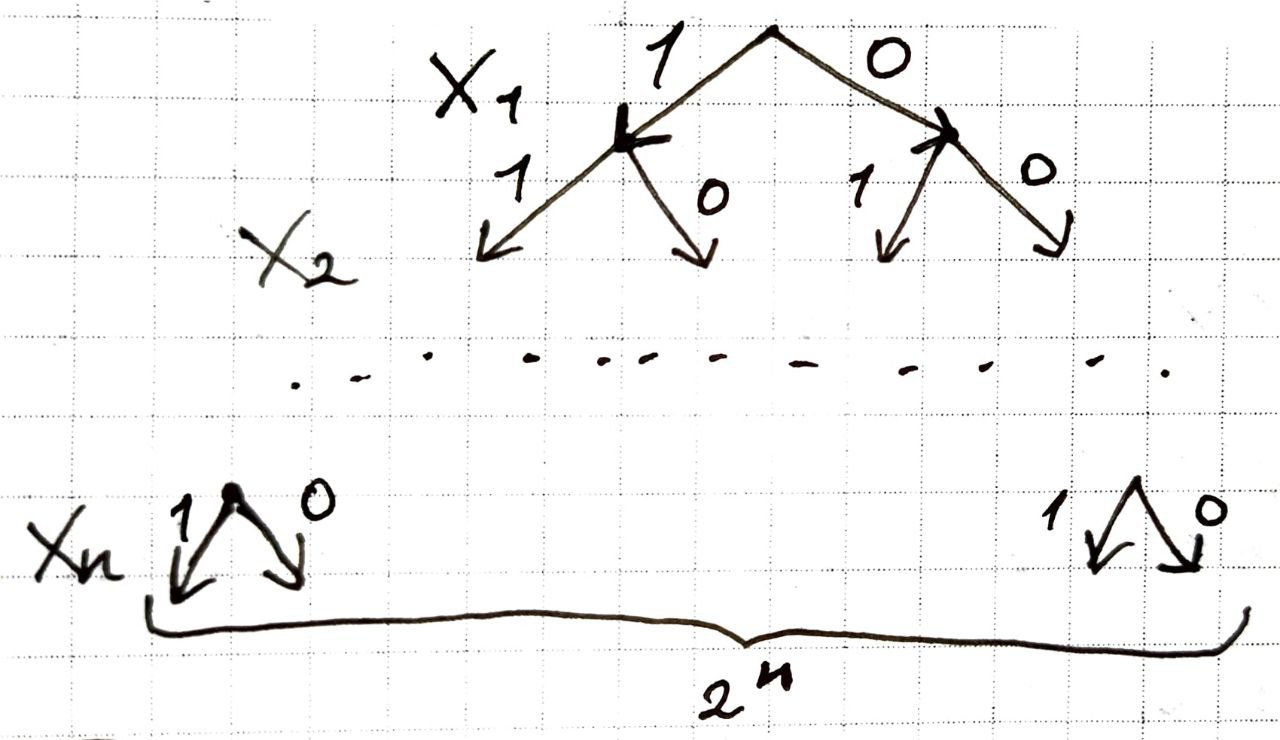
\includegraphics[height = 4cm]{images/kvain.jpg}
    \caption{Дерево перебора значений переменных}
\end{figure}

При этом используются основные тавтологии и следующие простейшие равенства:

$X\land1 = X$ \qquad $X\lor 1 = 1$ \qquad $0\Rightarrow X = 1$ \qquad $X\Rightarrow X = 1$

$X\land 0 = 0$ \qquad $X\lor 0 = X$ \qquad $1\Rightarrow X = X$ \qquad $X\Leftrightarrow X = 1$

$X\land\lnot X = 0$ \quad $X\lor\lnot X = 1$ \qquad $X\Rightarrow 1 = 1$  \qquad $X\Rightarrow 0 = \lnot X$

\begin{example}
    C помощью алгоритма Квайна выясните, является ли тождественно истинной формула
    $((Y\Rightarrow Z)\land(X\Rightarrow V)\land(X\lor\lnot Z))\Rightarrow(\lnot Y \lor V)$.

    1. При фиксировании в исходной формуле $X = 1$ получаем 
    
    $((Y\Rightarrow Z)\land(1\Rightarrow V)\land(1\lor\lnot Z))\Rightarrow(\lnot Y \lor V)$, что равносильно 
    
    $((Y\Rightarrow Z)\land V)\Rightarrow (\lnot Y\lor V)$.

    Положим здесь $Y = 1$: $((1\Rightarrow Z)\land V)\Rightarrow (\lnot 1\lor V)$, 
    
    что равносильно $(Z\land V)\Rightarrow V$.

    Отсюда при $Z = 1$ получаем $(1\land V)\Rightarrow V = V \Rightarrow V = 1$

    и при $Z = 0$ получаем $(0\land V)\Rightarrow V = 0 \Rightarrow V = 1$.

    Положим теперь $Y = 0$: $((0\Rightarrow Z)\land V)\Rightarrow(\lnot 0 \lor V) = V \Rightarrow 1 = 1$.
\\ \\
    2. При фиксированном в исходной формуле $X = 0$ получаем 

    $((Y\Rightarrow Z)\land(0\Rightarrow V)\land(0\lor\lnot Z))\Rightarrow(\lnot Y \lor V)$, что равносильно 
    
    $((Y\Rightarrow Z)\land\lnot Z) \Rightarrow (\lnot Y \lor V)$.

    Положим здесь $Y = 1$: $((1\Rightarrow Z)\land\lnot Z)\Rightarrow(\lnot 1 \lor V)$, что равносильно 
    
    $(Z\land\lnot Z)\Rightarrow V = 0 \Rightarrow V = 1$.

    Положим теперь $Y = 0$: $((0\Rightarrow Z)\land\lnot Z)\Rightarrow(\lnot 0\lor V)=\lnot Z \Rightarrow 1 = 1$.

    Таким образом, данная формула тождественно истинная.
\end{example}

Т.е. метод решения заключается в том, что для входящих в формулу пропозициональных переменных последовательно фиксируются возможные значения 0 или 1, и получившиеся формулы упрощаются с помощью перечисленных ранее простейших равенств до тех пор, пока не получается тождественно истинная формула 1.

При этом порядок фиксирования значений пропозициональных переменных может быть произвольным.

\begin{remark}
    Если на каком-то заключительном шаге вычислений получается не тождественно истинная формула 1, а тождественно ложная формула 0, то исследуемая формула не является тождественной истинной "--- она опровергается соответствующими фиксированными значениями пропозициональных переменных. 
\end{remark}

\subsection*{Алгоритм редукции}
\textit{Алгоритм редукции} используется при доказательстве тождественной истинности формулы с большим количеством импликаций. 

Идея метода основывается на получении противоречия из предположения, что истинное значение рассматриваемой формулы равно 0 при некоторых истинностных значениях ее пропозициональных переменных. 

При этом используется тот факт, что импликация ложна в том и только том случае, если ее посылка истинна и заключение ложно. 

\begin{example}
    С помощью алгоритма редукции выяснить, является ли тождественно истинной формула

    $((Y\Rightarrow Z)\land(X\Rightarrow V)\land(X\lor\lnot Z))\Rightarrow(\lnot Y\lor V)$.
    
    \textit{Решение.} Запишем по пунктам шаги алгоритма редукции.

    1. Предположим, что при некотором наборе значений переменных данная формула ложна, т.е. выполняется
$((Y\Rightarrow Z)\land(X\Rightarrow V)\land(X\lor\lnot Z))\Rightarrow(\lnot Y\lor V) = 0$, т.е. последняя импликация в ней ложна.

    2. По определению операции импликации это равносильно тому, что посылка импликации $(Y\Rightarrow Z)\land(X\Rightarrow V)\land(X\lor\lnot Z) = 1$ и ее следствие $\lnot Y\lor V = 0$.

    3. По определению операций конъюнкции и дизъюнкции это равносильно тому, что $Y\Rightarrow Z = 1$, $X\Rightarrow V = 1$, $X\lor\lnot Z = 1$ и $\lnot Y = 0$, $V = 0$.

    4. Отсюда по определению операции отрицания получаем, что $Y = 1$.
    
    5. Тогда по определению операции импликации из первого равенства пункта 3 следует $Z = 1$ и из второго равенства этого пункта следует $X = 0$.

    6. Отсюда по определению операции отрицания получаем, что $\lnot Z = 0$.

    7. Подставляя найденные значения $X = 0,\lnot Z = 0$ в формулу $X\lor\lnot Z$, по определению операции дизъюнкции получаем условие $X\lor\lnot Z = 0$, которое противоречит третьему равенству пункта 3.

    Значит, наше предположение неверно и данная формула является тождественно истинной.
\end{example}

\begin{figure}[H]
    \centering
    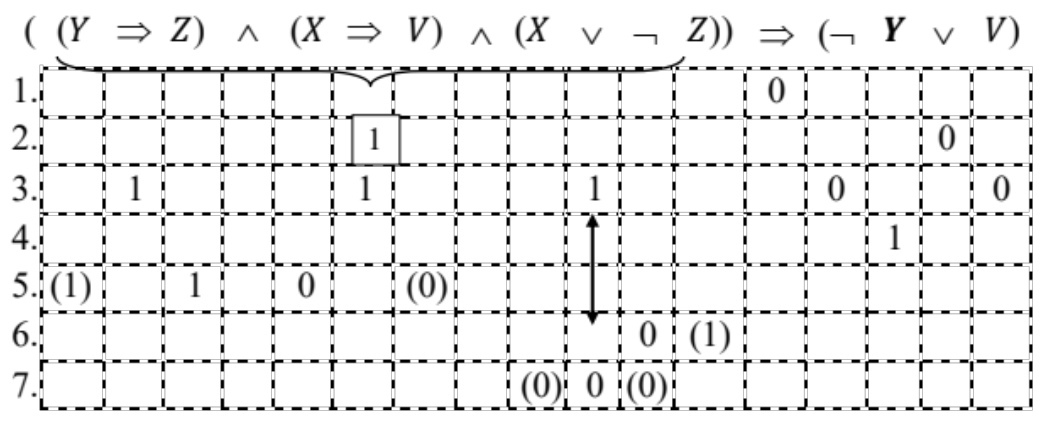
\includegraphics[height = 3cm]{images/reducto.jpg}
    \caption{На каждом шаге алгоритма в скобках указываются значения переменных, которые были получены ранее на предыдущих шагах вычислений}
\end{figure}

\subsection*{Метод семантических таблиц в алгебре высказываний}
\begin{definition}
    \textit{Оценкой переменных} в формуле $\Phi = \Phi(X_1,\ldots,X_n)$ называется отображение $\alpha$ множества $\{X_1,\ldots,X_n\}$ в множестве $\{0,1\}$.
    Обозначения: $\models_a\Phi$ и $\nvDash_a \Phi$.
\end{definition}
\begin{definition}
    \textit{Семантической таблицей} называется упорядоченная пара множества формул $\langle\Gamma |\Delta  \rangle $.

    Семантическая таблица $\langle\Gamma |\Delta  \rangle $ называется \textit{выполнимой}, если существует такая оценка переменных $a$, что
    \begin{enumerate}
        \item $\Phi\models_a$ для любой формулы $\Phi \in \Gamma$
        \item $\Uppsi\nvDash_a$ для любой формулы $\Uppsi\in\Delta$
    \end{enumerate}
\end{definition}

\begin{example}
    Семантическая таблица $\langle \{X,\lnot Y\} | \{X\Rightarrow Y\} \rangle $ выполнима для оценки $a(X) = 1, a(Y) = 0$.
\end{example}

\begin{example}
    Семантическая таблица $\langle \varnothing | \{X \lor\lnot X\} \rangle $ невыполнима.
\end{example}

\begin{theorem}[Основная теорема метода семантических таблиц]
    Для любой формулы $\Phi$ условие $\models \Phi$ выполняется тогда и только тогда, когда семантическая таблица $\langle \varnothing | \{\Phi\} \rangle $ невыполнима.
\end{theorem}

\begin{example}
    С помощью семантических таблиц докажем тождественную истинность формулы $\Phi = ((X\Rightarrow Y)\Rightarrow X)\Rightarrow X$, которая называется \textit{законом Пирса}.
\end{example}

Табличный вывод семантической таблицы $T_0 = \langle \varnothing | \Phi \rangle $:
\begin{figure}[H]
    \centering
    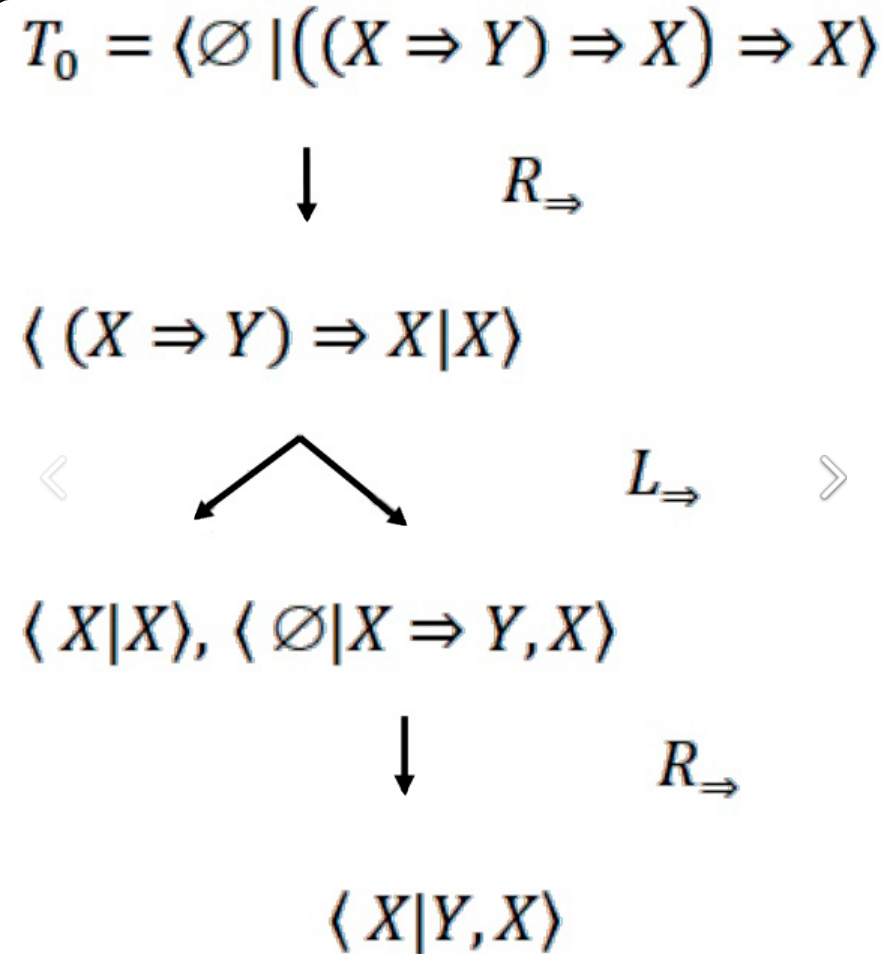
\includegraphics[height = 4cm]{images/pirse.png}
\end{figure}

(Про эти штуки есть еще немного в конспектах, но в целом зачем?..)


\section{Метод резолюций в логике высказываний}
\subsection*{Метод резолюций в алгебре высказываний}
Следующие задачи равносильны:
\begin{enumerate}
    \item Проверка тождественной истинности формул
    \item Проверка логического следования формул
    \item Проверка тождественной ложности формул
    \item Проверка противоречивости множества формул
    \item Проверка противоречивости множества дизъюнктов
\end{enumerate}

\begin{definition}
    Пусть для некоторой переменной $X$ дизъюнкты $D_1, D_2$ представимы в виде $D_1=D_1'\lor X$, $D_2=D_2'\lor\lnot X$. Тогда дизъюнкт $D_1'\lor D_2'$ называется \textit{резовльвентой дизъюнктов} $D_1,D_2$ по переменной $X$ и обозначается $\text{Res}_X(D_1,D_2)$.

    Резольвента дизъюнктов $D_1,D_2$ по некоторой переменной $X$ называется \textit{резольвентой дизъюнктов} $D_1,D_2$ и обозначается Res$(D_1,D_2)$. 
    
    По определению Res$(X,\lnot X) = 0$.
\end{definition}

\textbf{Свойство.} Если $D_1=D_1'\lor X$, $D_2=D_2'\lor\lnot X$ выполнимы, то выполнима Res$_X(D_1,D_2)$.

\begin{definition}
    \textit{Резолютивным выводом формулы} $\Phi$ из множества дизъюнктов $S=\{D_1,\ldots,D_m\}$ называется такая последовательность формул $\Phi_1,\ldots,\Phi_n$, что:
    \begin{enumerate}
        \item $\Phi_n = \Phi$
        \item Каждая из формул $\Phi_i$ $(i=1,\ldots,n)$ либо принадлежит множеству $S$, либо является резолвьентой $\Phi_i=$ Res$(\Phi_j,\Phi_k)$ предыдущих формул $\Phi_j$, $\Phi_k$ при некоторых $1\leq j$, $k\leq i$.
    \end{enumerate}
\end{definition}

\begin{theorem}[Основная теорема метода резолюций]
    Множество дизъюнктов $S = \{D_1,\ldots,D_m\}$ противоречиво в том и только том случае, если существует резолютивный вывод значения 0 из множества $S$.
    
    Так как по критерию логического следования соотношение 
    $$\Phi_1,\ldots,\Phi_m\models \Phi$$ равносильно условию $$\Phi_1,\ldots,\Phi_m,\lnot\Phi\models,$$ то справедлив следующий результат.
\end{theorem}

\begin{corollary}[Проверка логического следования формул]
    Пусть для формул $\Phi_1,\ldots,\Phi_n,\Phi$ формула $\Uppsi=\Phi_1\land\ldots\land\Phi_n\land\lnot\Phi$ имеет КНФ \\ $\Uppsi=D_1\land\ldots\land D_m$.

    Тогда логическое следование $\Phi_1,\ldots,\Phi_n\models\Phi$ равносильно существованию резолютивного вывода значения 0 из множества дизъюнктов $S=\{D_1,\ldots,D_m\}$.
\end{corollary}

\subsection*{Алгоритм проверки логического следования формул $\Phi_1,\ldots\Phi_n\models\Phi$:}
\begin{enumerate}
    \item Составить формулу $\Uppsi=\Phi_1\land\ldots\land\Phi_n\land\lnot\Phi$ и найти ее КНФ \\ $\Uppsi=D_1\land\ldots\land D_m$.
    \item Найти резолютивный вывод значения 0 из множества $S = \{D_1,\ldots,D_m\}$.
    \item Если такой вывод существует, то выполняется $\Phi_1,\ldots,\Phi_n\models \Phi$.
\end{enumerate}

\begin{example}
    Методом резолюций проверим логическое следование: \\
    $(\lnot X\Rightarrow Z),(Y\Rightarrow W),((W\land Z)\Rightarrow V), (\lnot V) \models X \lor \lnot Y$

    Данное соотношение равносильно условию \\
    $(\lnot X\Rightarrow Z),(Y\Rightarrow W),((W\land Z)\Rightarrow V), (\lnot V), \lnot (X\lor\lnot Y)\models$, \\т.е. условию противоречивости формулы \\
    $\Uppsi = (\lnot X\Rightarrow Z)\land(Y\Rightarrow W)\land((W\land Z)\Rightarrow V)\land (\lnot V)\land \lnot (X\lor\lnot Y)$.

    Найдем КНФ этой формулы:
    $\Uppsi=(X\lor Z)\land(\lnot Y\lor W)\land (\lnot(W\land Z)\lor V)\land\lnot V\land(\lnot X\land Y) = (X\lor Z)\land(\lnot Y\lor W)\land(\lnot W\lor\lnot Z\lor V)\land\lnot V\land\lnot X\land Y$.

    Рассмотрим множество дизъюнктов \\
    $S = \{X\lor Z,\lnot Y\lor W,\lnot W\lor\lnot Z\lor V,\lnot V,\lnot X, Y\}$. Построим резолютивный вывод значения 0 из этого множества $S$:

    $\Phi_1 = $ Res$_X(X\lor Z,\lnot X) = Z$

    $\Phi_2 = $ Res$_Y(\lnot Y\lor W,Y) = W$

    $\Phi_3 = $ Res$_Z(\lnot W\lor\lnot Z\lor V, Z) = \lnot W \lor V$

    $\Phi_4 = $ Res$_W(\Phi_2,\Phi_3) = V$

    $\Phi_5 = $ Res$(\Phi_4\lnot V) = 0$

    Таким образом, множество дизъюнктов формулы $\Uppsi$ противоречиво и, значит, выполняется исходное логическое следование.
\end{example}

\subsection*{Алгоритм проверки тождественной истинности формулы Ф:}
1.Рассмотреть формулу $\Uppsi=\lnot \Phi$ и найти ее КНФ $\Uppsi = D_1\land\ldots\land D_m$.

2. Найти резолютивный вывод значения 0 из множества $S = \{D_1,\ldots,D_m\}$.

3. Если такой вывод существует, то выполняется $\models\Phi$.

\begin{example}
    Методом резолюций проверить тождественную истинность формулы 
    $$\Phi=(X\Rightarrow Y)\Rightarrow((X\Rightarrow\lnot Y)\Rightarrow\lnot X)$$
    \textbf{Решение.} По критерию логического следования тавтологии $\models \Phi$ равносильности противоречивости формулы: $$\Uppsi = \lnot\Phi = \lnot((X\Rightarrow Y)\Rightarrow ((X\Rightarrow\lnot Y)\Rightarrow\lnot X)).$$

    Найдем КНФ этой формулы $$\Uppsi = \lnot(\lnot(\lnot X\lor Y)\lor(\lnot(\lnot X\lor\lnot Y)\lor\lnot X)) = (\lnot X\lor Y)\land(\lnot X\lor\lnot Y)\land X.$$

    Рассмотрим множество дизъюнктов полученной КНФ формулы $\Uppsi$:
    $$S = \{\lnot X\lor Y,\lnot X\lor\lnot Y, X\}$$.

    Построим резолютивный вывод значения 0 из этого множества $S$:

    $\Phi_1 = \lnot X\lor Y$

    $\Phi_2 = \lnot X\lor\lnot Y$

    $\Phi_3 =$ Res$_Y(\Phi_1,\Phi_2) =$ Res$_Y(\lnot\lor Y,\lnot X\lor\lnot Y) = \lnot X\lor\lnot X = \lnot X$ 

    $\Phi_4 = X$

    $\Phi_5 = $ Res$(\Phi_3,\Phi_4) = $ Res$(\lnot X, X) = 0$

    Таким образом, из множества дизъюнктов $S$ резолютивно выводится значение 0 и по основной теореме множество $S$ противоречиво. 

    Следовательно, формула $\Uppsi$ противоречива и выполняется $\models\Phi$.
\end{example}

\section{Понятие предиката и его множества истинности. Перенесение на предикаты логических операций}
%\section{Понятие предиката и его множества истинности. Перенесение на предикаты логических операций}

%\section{Кванторы общности и существования, их действие на предикат. Свободные и связанные переменные}

%\section{Формулы алгебры предикатов}

%\section{Интерпретация формул алгебры предикатов}

\subsection*{Логика предикатов. Понятие предиката.}
Выразительные средства алгебры высказываний недостаточны для описания утверждений со сложной логической структурой субъектно-предикатных рассуждений, в которых используются не только понятие \textit{субъекта} (как объекта, о котором говорится в рассуждении), но и понятие \textit{предиката} (как выраженного сказуемыми свойства объектов рассуждения).

\begin{definition}
    \textit{Предикатом} называется утверждение, содержащее переменные $x_1,\ldots,x_n$, которое превращается в высказывание при замене этих переменных конкретными объектами из некоторой области возможных значений.

    Обозначаются предикаты $P,Q,\ldots$
\end{definition}

\begin{definition}
    Переменные $x_1,\ldots,x_n$ называются \textit{предметными} или \textit{индивидуальными переменными}. Число предметных переменных в предикате называется его \textit{арностью} или \textit{местностью}.

    Более точно, предикат $P$ с $n$ предметными переменными называется \textit{n-арным} или \textit{n-местным предикатом} и обозначается $P(x_1,\ldots,x_n)$.
\end{definition}

Предикат $P(x_1,\ldots,x_n)$ является функцией, которая каждому набору значений $x_1=a_1,\ldots,x_n=a_n$ его $n$ предметных переменных $x_1,\ldots,x_n$ ставит в соответствие некоторое высказывание $P(a_1,\ldots,a_n)$, имеющее определенное истинностное значение $\lambda(P(a_1,\ldots,a_n))$.

Если отвлечься от содержания высказываний и учитывать только их истинностные значения, то предикат можно рассматривать как функцию со значениями в множестве $\{0,1\}$.

Рассматривая такую функцию на некотором фиксированном множестве $M$ допустимых значений предметных переменных предиката, получим $n-$арное отношение на множестве $M$, состоящее из всех таких упорядоченных наборов $(a_1,\ldots,a_n)$ $n$ элементов $a_1,\ldots,a_n\in M$, для которых $P(a_1,\ldots,a_n)$ является истинным высказыванием.

Такое $n-$арное отношение обозначается символом $P^+$ и называется \textit{множеством истинности} предиката $P$ на множестве $M$. \\ \\ \\

Функция $P:M^n\rightarrow \{0,1\}$ определяется двумя множествами:

\begin{enumerate}
    \item \textit{Множество истинности: } 
    $$P^+=\{(a_1,\ldots,a_n)\in M^n:\lambda(P(a_1,\ldots,a_n))=1\}$$
    \item \textit{Множество ложности:} $$P^-=\{(a_1,\ldots,a_n)\in M^n:\lambda(P(a_1,\ldots,a_n))=0\}$$
\end{enumerate}

\begin{example}
    Пусть $M - $ множество студентов вуза.

    Предикаты:

    $P(x) - $ <<x есть студент 1-ой группы>>,

    $Q(x) - $ <<студент x есть отличник>>.

    Множеством истинности $P^+$ на множестве $M$ является множество студентов 1-ой группы вуза и множеством истинности $Q^+$ на множестве $M$ является множество всех отличников вуза.
\end{example}

\begin{example}
    Пусть $M - $ множество вещественных чисел $\mathbb{R}$.

    Предикаты:

    $P(x) - $ утверждение <<x>0>>,

    $Q(x) - $ утверждение <<$(x-1)(x^2-2) = 0$>>.

    Множеством истинности предиката $P$ на множестве $M = \mathbb{R}$ является множество всех положительных вещественных чисел и множеством истинности предиката $Q$ на множестве $M = \mathbb{R} $ является множество \\
    $Q^+ = \{1,\sqrt{2},-\sqrt{2}\}$.
\end{example}

\begin{definition}
    Предикат $P(x_1,\ldots,x_n)$ на множестве $M$ называется:

    \begin{itemize}
        \item \textit{Тождественно истинным}, если для любых значений $x_1=a_1\in M,\ldots,x_n=a_n \in M$ высказывание $P(a_1,\ldots,a_n)$ истинно, т.е. $P^+=M^n$.
        \item \textit{Тождественно ложным}, если для любых значений $x_1=a_1 \in M,\ldots,x_n=a_n \in M$ высказывание $P(a_1,\ldots,a_n)$ ложно, т.е. $P^+=\varnothing$.
        \item \textit{Выполнимым}, если для некоторых значений $x_1=a_1 \in M,\ldots,x_n=a_n \in M$ высказывание $P(a_1,\ldots,a_n)$ истинно, т.е. $P^+\neq \varnothing$.
        \item \textit{Опровержимым}, если для некоторых значений $x_1=a_1 \in M,\ldots,x_n=a_n \in M$ высказывание $P(a_1,\ldots,a_n)$ ложно, т.е. $P^+\neq M^n$.
    \end{itemize}
\end{definition}

\subsection*{Алгебра предикатов}
\begin{definition}
    \textit{Отрицание $n-$местного предиката $P(x_1,\ldots,x_n)$} определяется как $n-$местный предикат $\lnot P$, который при подстановке значений $x_1=a_1,\ldots,x_n=a_n$ превращается в высказывание $\lnot P(a_1,\ldots,a_n)$, являющееся отрицанием высказывания ${P(a_1,\ldots,a_n)}$.
\end{definition}

\begin{definition}
    \textit{Конъюнкция $n-$местных предикатов $P(x_1,\ldots,x_n)$ и $Q(x_1,\ldots,x_n)$} определяется как $n-$местный предикат $P\land Q$, который при подстановке значений $x_1=a_1,\ldots,x_n=a_n$ превращается в высказывание $P\land Q(a_1,\ldots,a_n)$, являющееся конъюнкцией высказываний $P(a_1,\ldots,a_n)$ и $Q(a_1,\ldots,a_n)$.
\end{definition}

Для любого множества $M$ допустимых значений предметных переменных предикатов множества истинности предикатов взаимосвязаны с логическими операциями по следующим формулам:

$(\lnot P)^+=M^n \backslash P+$

$(P\land Q)^+ = P^+\cap Q^+ $

$(P\lor Q)^+=P^+\cup Q^+$

$(P\Rightarrow Q)^+=(\lnot P)^+\cup Q^+$

$(P\Leftrightarrow Q)^+ = (P\Rightarrow Q)^+\cap(Q\Rightarrow P)^+$

\begin{example}
    Пусть на множестве вещественных чисел $\mathbb{R} $ предикат $P(x)$ выражается неравенством $f(x)\leq 0,$ и предикат $Q(x)$ выражается неравенством $g(x)\leq 0$.

    Тогда система неравенств
         $\begin{cases} f(x)\leq 0 \\ g(x)\leq 0 \end{cases}$
    определяется как конъюнкция предикатов $P\land Q$ и, значит, имеет множество решений $(P\cap Q)^+=P^+\cap Q^+$, равное пересечению множеств решений неравенств системы.

    Совокупность неравенств 
    $\left[ 
      \begin{gathered} 
        f(x)\leq 0, \\ 
        g(x)\leq 0 \\ 
      \end{gathered} 
\right.$ определяется как дизъюнкция предикатов $P\lor Q$ и, значит, имеет множество решений $(P\cup Q)^+=P^+\cup Q^+$, равное объединению множеств решений неравенств системы.
\end{example}


\section{Кванторы общности и существования, их действие на предикат. Свободные и связанные переменные}

\section{Формулы алгебры предикатов}

\section{Интерпретация формул алгебры предикатов}

\section{Логическое равенство формул алгебры предикатов. Свойства логических операций над предикатами}

\section{Логическое следование формул алгебры предикатов}

\section{Предваренная нормальная форма (ПНФ) формул алгебры предикатов}

\section{Скулемовская стандартная форма (ССФ) формул алгебры предикатов}

\section{Сведение проблемы общезначимости формул к проблеме противоречивости систем дизъюнктов}

\section{Унификация формул}

\section{Метод резолюций в логике предикатов}

\section{Аксиомы и правила вывода исчисления высказываний. Доказуемость формул}

\section{Теорема Геделя о полноте исчисления высказываний}

\section{Непротиворечивость и разрешимость исчисления высказываний}

\section{Аксиомы и правила вывода исчисления предикатов. Тождественная истинность выводимых формул}

\section{Полнота, непротиворечивость и неразрешимость исчисления предикатов}

\section{Понятие алгоритма и основные математические модели алгоритма}

\section{Разрешимые и полуразрешимые языки. Теорема Поста}

\section{Машины Тьюринга и вычисляемые ими функции}

\section{Распознаваемость языков машинами Тьюринга}

\section{Разрешимые, неразрешимые и распознавательные проблемы}

\section{Временная и ленточная сложность машины Тьюринга}

\section{Классы языков P и NP}

\section{Полиномиальные сведения проблем}

\section{NP"=трудные и NP"=полные языки}

\section{Основные NP"=полные проблемы}

\end{document}